\documentclass{article}

\usepackage{graphicx}
\usepackage{booktabs}
\usepackage{tabularray}
\usepackage{float}
\usepackage{graphicx}
\usepackage{codehigh}
\usepackage[normalem]{ulem}
\UseTblrLibrary{booktabs}
\UseTblrLibrary{siunitx}
\newcommand{\tinytableTabularrayUnderline}[1]{\underline{#1}}
\newcommand{\tinytableTabularrayStrikeout}[1]{\sout{#1}}
\NewTableCommand{\tinytableDefineColor}[3]{\definecolor{#1}{#2}{#3}}

\title{Mini Research Project}
\author{Your Name}
\date{}

\begin{document}

\maketitle

I am using the presidential approval database and running two different models 
for my analisis

\section*{Regression Results}

\begin{table}
\centering
\begin{tblr}[         %% tabularray outer open
]                     %% tabularray outer close
{                     %% tabularray inner open
colspec={Q[]Q[]Q[]},
hline{2}={1-3}{solid, black, 0.05em},
hline{12}={1-3}{solid, black, 0.05em},
hline{1}={1-3}{solid, black, 0.08em},
hline{20}={1-3}{solid, black, 0.08em},
column{2-3}={}{halign=c},
column{1}={}{halign=l},
}                     %% tabularray inner close
& Simple Model & With Controls \\
(Intercept) & \num{57.094} & \num{59.616} \\
& (\num{2.082}) & (\num{4.266}) \\
UnemPct & \num{-0.923} & \num{-3.436} \\
& (\num{0.362}) & (\num{0.343}) \\
DemPct &  & \num{0.265} \\
&  & (\num{0.075}) \\
RepPct &  & \num{-0.190} \\
&  & (\num{0.079}) \\
factor(PARTY)2 &  & \num{17.551} \\
&  & (\num{1.131}) \\
Num.Obs. & \num{492} & \num{492} \\
R2 & \num{0.013} & \num{0.352} \\
R2 Adj. & \num{0.011} & \num{0.346} \\
AIC & \num{3988.8} & \num{3788.1} \\
BIC & \num{4001.4} & \num{3813.3} \\
Log.Lik. & \num{-1991.378} & \num{-1888.034} \\
F & \num{6.516} & \num{66.032} \\
RMSE & \num{13.85} & \num{11.23} \\
\end{tblr}
\end{table}


\section*{Figure}

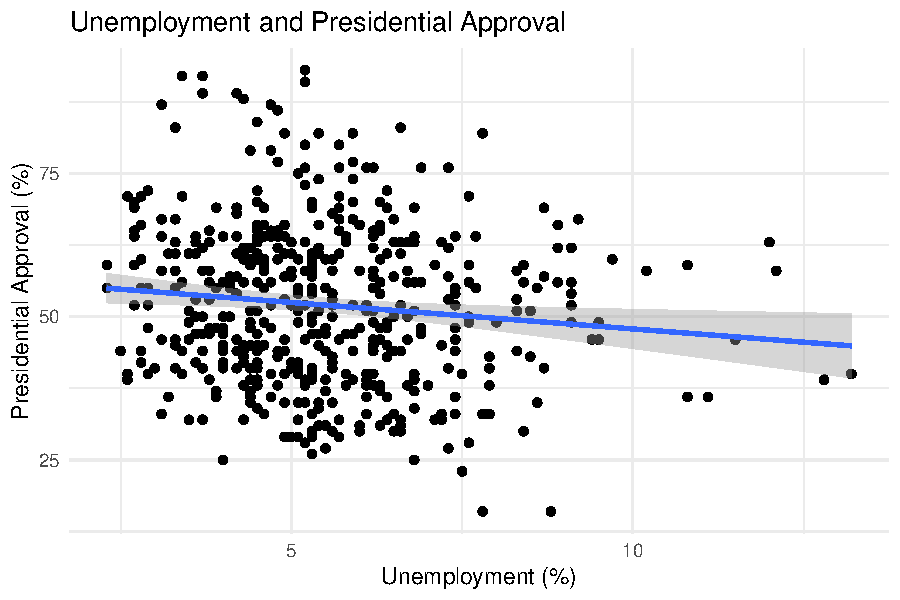
\includegraphics[width=0.8\textwidth]{img/scatter_plot.pdf}

\end{document}